% Citation début de chapitre
\dictum[Schiller]{So pause ye who would link your fates~\dots}%

\chaptertoc{}

\addsec{Introduction}

Introduction du chapitre

% \cite{Bunel2018}

\section{Secours en montagne}

Le secours en montagne est partagé entre les \glspl{pghm} et les \glspl{pgm},
\gls{crsm}. les \glspl{pghm} et les \glspl{crsm} ne peuvent pas se blairer.

Comme le disait le matcho, Roger Brunet : \enquote{L'espace
  géographique ne se découpe pas plus arbitrairement qu'un poulet à
  table.} Ce qui est, on peut le dire, une véritable \emph{punchline}
géographique.

Malgré des sigles identiques, il convient de ne pas confondre le
\glspl{TCP1} et le \gls{TCP2}.

\begin{carte}
  \begin{center}
    \begin{tikzpicture}
\node[inner sep=0pt, anchor=south west] (image) at (0,0){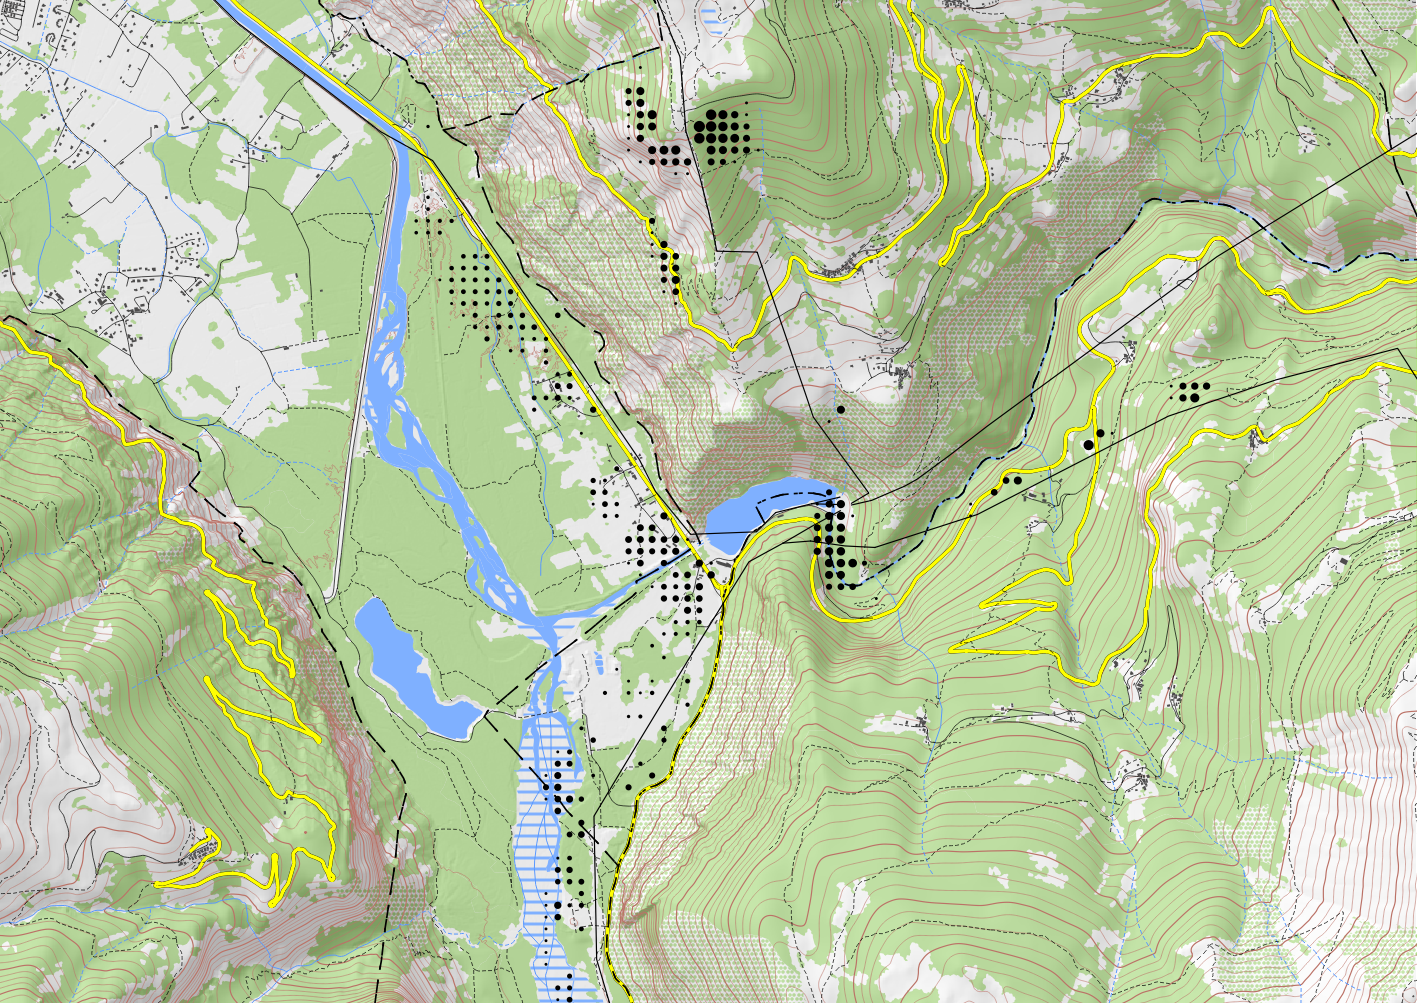
\includegraphics{./figures/CarteTest.png}};
\begin{scope}
\node (P2) at ([yshift=-.5cm]image.south east) {};
\node (P1) at ([yshift=-.5cm]image.south west) {};

% \draw[-] (P1) -- (P2);

\foreach \xshift/\diam in {0/.05, .1/.04, .2/.03, .3/.02, .4/.01}
{
\draw[fill=black,draw=none] ([xshift=\xshift cm, yshift=-.5cm]P1) circle [radius=\diam cm];
}

% Légende détaillée
\path (P1) -- (P2) node[pos=.5, yshift=-.5cm] {\tiny Pour la légende détaillée du fond topographique voir \autoref{anx:topo_leg}}; 

% Échelle
\draw[-] (P2 |- -1cm,-1cm) --++ (-1,0) node[pos=.5, above] {\footnotesize\SI{500}{\meter}};
\end{scope}
\end{tikzpicture}
  \end{center}
  \caption{Représentation de la}
  \label{fig:1}
\end{carte}

\subsection{Cartographie}

\blindtext

\begin{carte}
  \begin{center}
    \begin{tikzpicture}
      \tikzset{et/.style={above,font=\vphantom{Ag}}}
      
      \node[inner sep=0pt, anchor=south west] (image) at (0,0){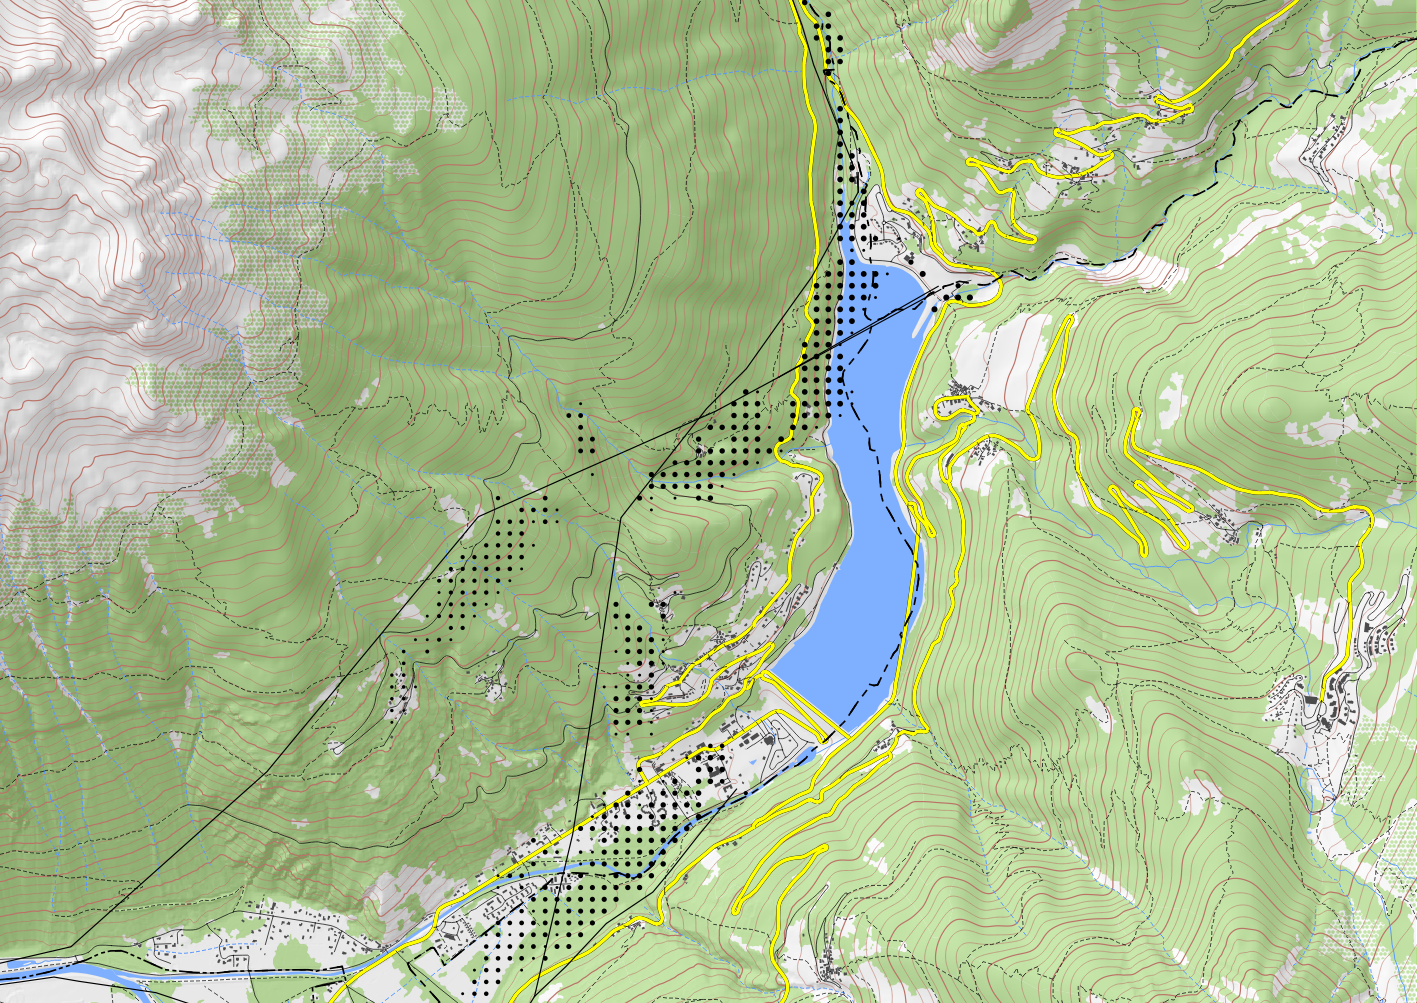
\includegraphics{./figures/CarteTest2.png}};
      
      \begin{scope}
        \node (P2) at ([yshift=-.5cm]image.south east) {};
        \node (P1) at ([yshift=-.5cm]image.south west) {};
        
        \foreach \x [evaluate=\xshift using \x/10, evaluate=\rad using (\x * .0004) + .01] in {0,...,100}
        {
          \draw[fill=black,draw=none, below] ([xshift=\xshift cm, yshift=-.5cm]P1) circle [radius=\rad cm];
        }

        \path(P1 |- 0cm,-1cm) --++ (10,0)
        node[et,pos=0] {0}
        node[et,pos=.1] {0,1}
        node[et,pos=.2] {0,2}
        node[et,pos=.3] {0,3}
        node[et,pos=.4] {0,4}
        node[et,pos=.65] {0,65}
        node[et,pos=1] {1};
        
        % Échelle
        \draw[-] (P2 |- -1cm,-1cm) --++ (-1,0) node[et,pos=.5] {\SI{500}{\meter}};

        % Légende détaillée
        \path (P1) -- (P2) node[pos=.5, yshift=-1cm] {\tiny Pour la légende détaillée du fond topographique voir \autoref{anx:topo_leg}. Sources: BD TOPO 2018, BD ALTI 2018.}; 
      \end{scope}
    \end{tikzpicture}
  \end{center}
  \caption{Représentation de la}
  \label{fig:1}
\end{carte}

\blindtext

\subsubsection{Cartographie bis}

\blindtext

\paragraph{Pragraphe test}

\blindtext

\subparagraph{Pragraphe test}

\blindtext

\begin{carte}
  \begin{center}
    \begin{tikzpicture}
      \tikzset{
        et/.style={above,font=\vphantom{Ag}},
        etv/.style={right,font=\vphantom{Ag}}}
      
      \node[inner sep=0pt, anchor=south west] (image) at (0,0){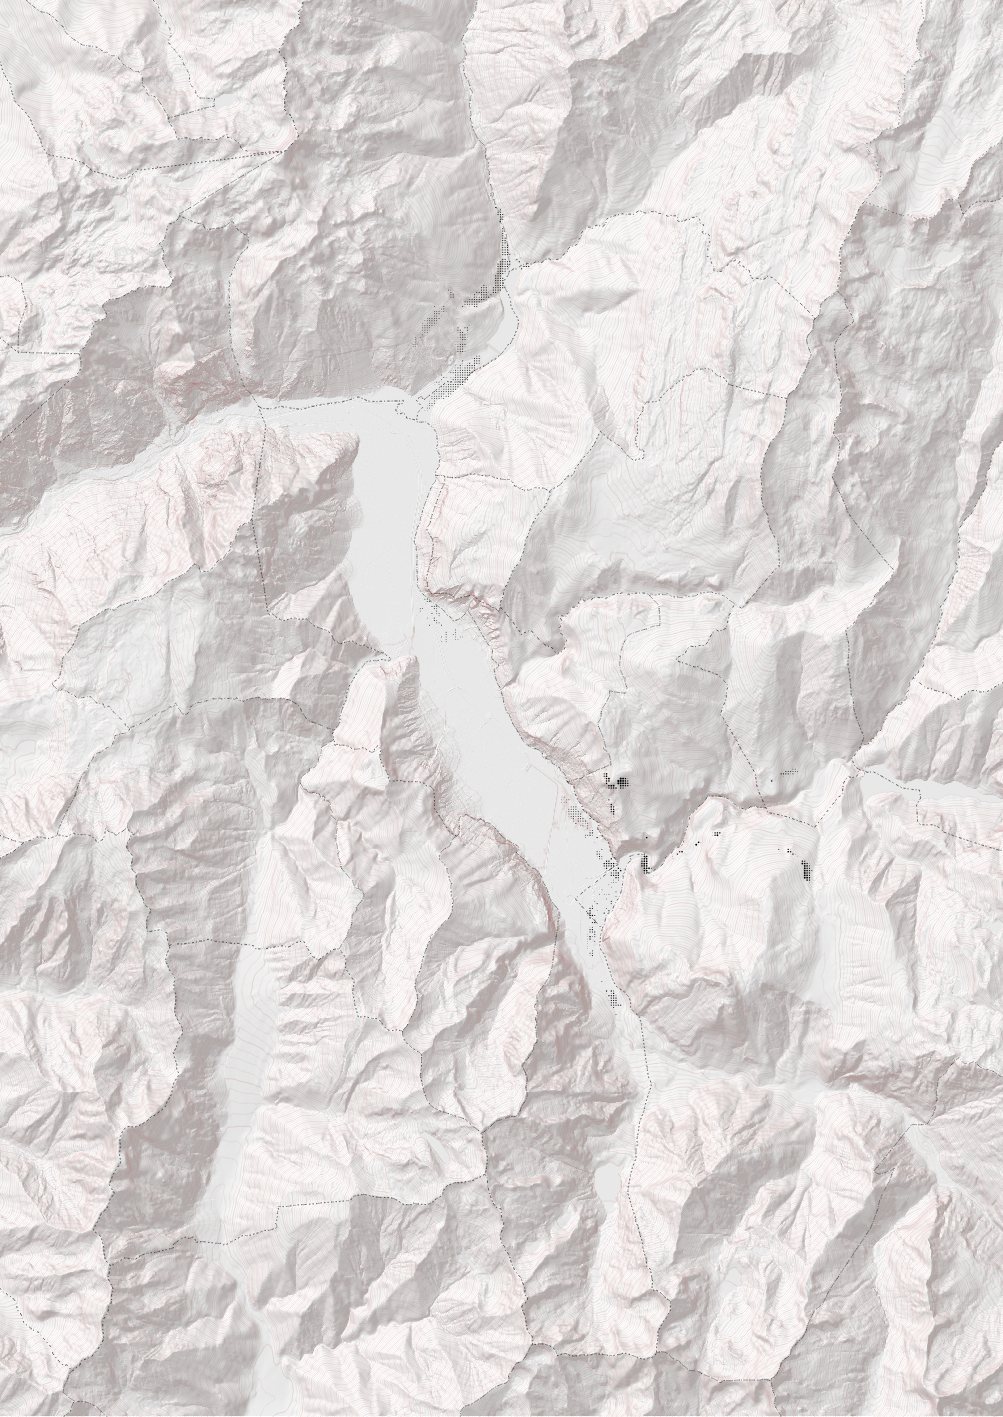
\includegraphics{./figures/CarteTest3.png}};
      
      \begin{scope}
        \node (P1) at ([xshift=.5cm]image.north east) {};
        \node (P2) at ([xshift=.5cm]image.south east) {};
        
        \foreach \y [evaluate=\yshift using \y/10, evaluate=\rad using (\y * .0004) + .01] in {0,...,100}
        {
          \draw[fill=black,draw=none, below] ([yshift=-\yshift cm]P1) circle [radius=\rad cm];
        }

        \path(P1) --++ (0,-10cm)
        node[etv,pos=0] {0}
        node[etv,pos=.1] {0,1}
        node[etv,pos=.2] {0,2}
        node[etv,pos=.3] {0,3}
        node[etv,pos=.4] {0,4}
        node[etv,pos=.65] {0,65}
        node[etv,pos=1] {1};
        
        % Échelle
        \draw[-] (P2 |- 1cm,0) --++ (1,0) node[et,pos=.5] {\SI{500}{\meter}};

        % Légende détaillée
        \path (image.south west) -- ([xshift=1cm]image.south east) node[pos=.5, yshift=-.5cm] {\tiny Pour la légende détaillée du fond topographique voir \autoref{anx:topo_leg}. Sources: BD TOPO 2018, BD ALTI 2018.}; 
      \end{scope}
    \end{tikzpicture}
  \end{center}
  \caption{Représentation de la}
  \label{fig:1}
\end{carte}


\blindtext

\begin{carte}
  \begin{center}
    \begin{tikzpicture}
      \node[inner sep=0pt, anchor=south west] (image) at (0,0){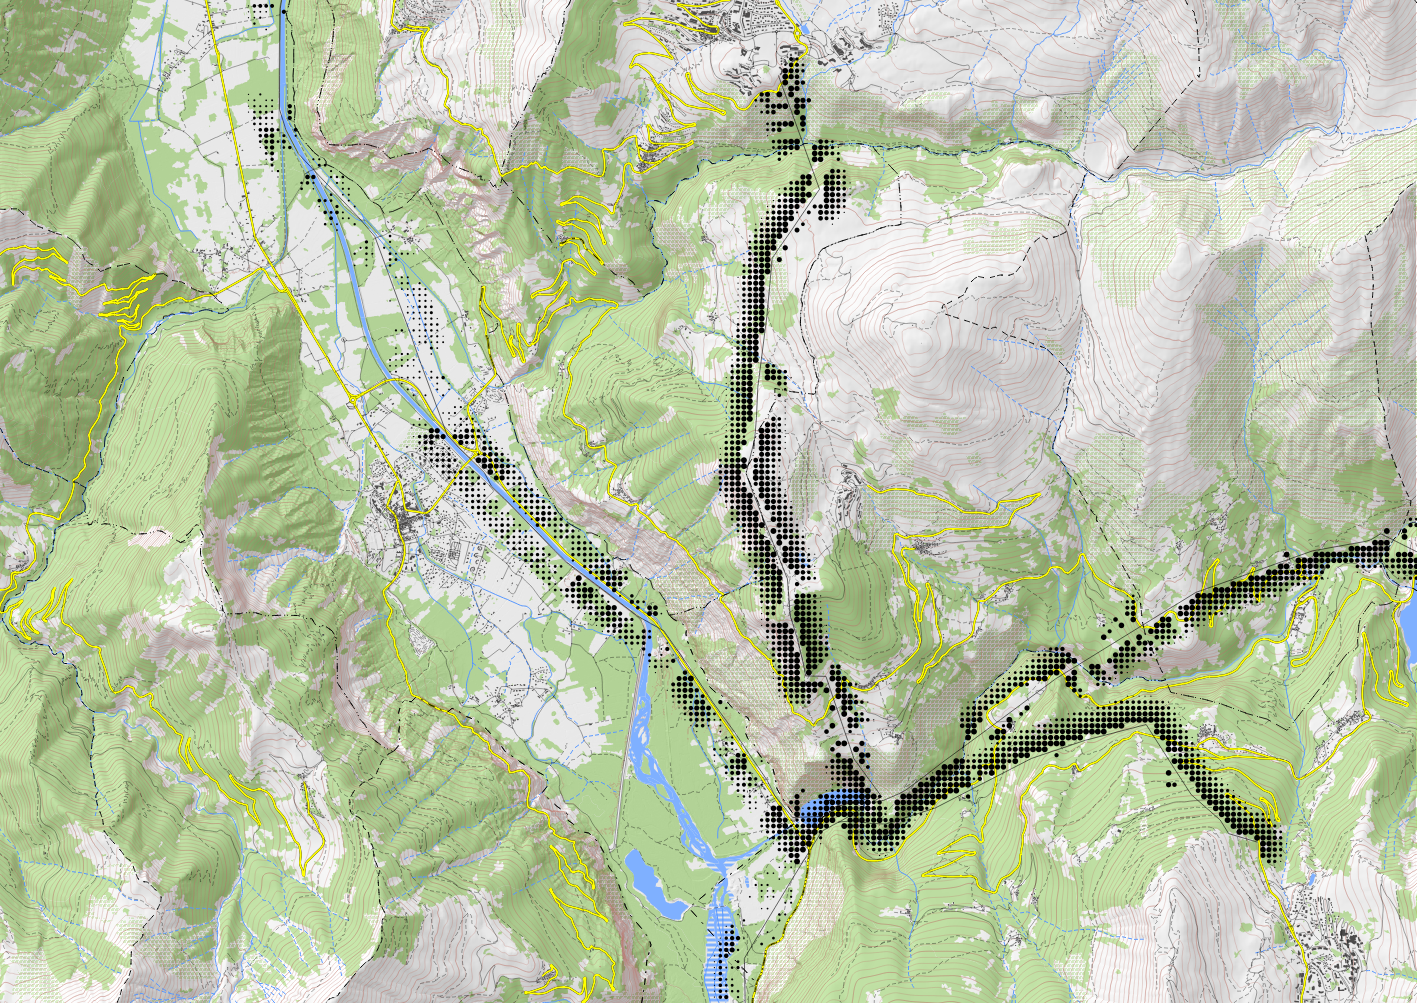
\includegraphics{./figures/CarteTest4.png}};
      \begin{scope}[yshift=-.5cm]
        \draw[-] (image.south east |- 0,0) -- (image.south west |- 0,0);
      \end{scope}
    \end{tikzpicture}
  \end{center}
  \caption{Représentation de la}
  \label{fig:1}
\end{carte}

\begin{carte}
  \begin{center}
    \begin{tikzpicture}
      \node[inner sep=0pt, anchor=south west] (image) at (0,0){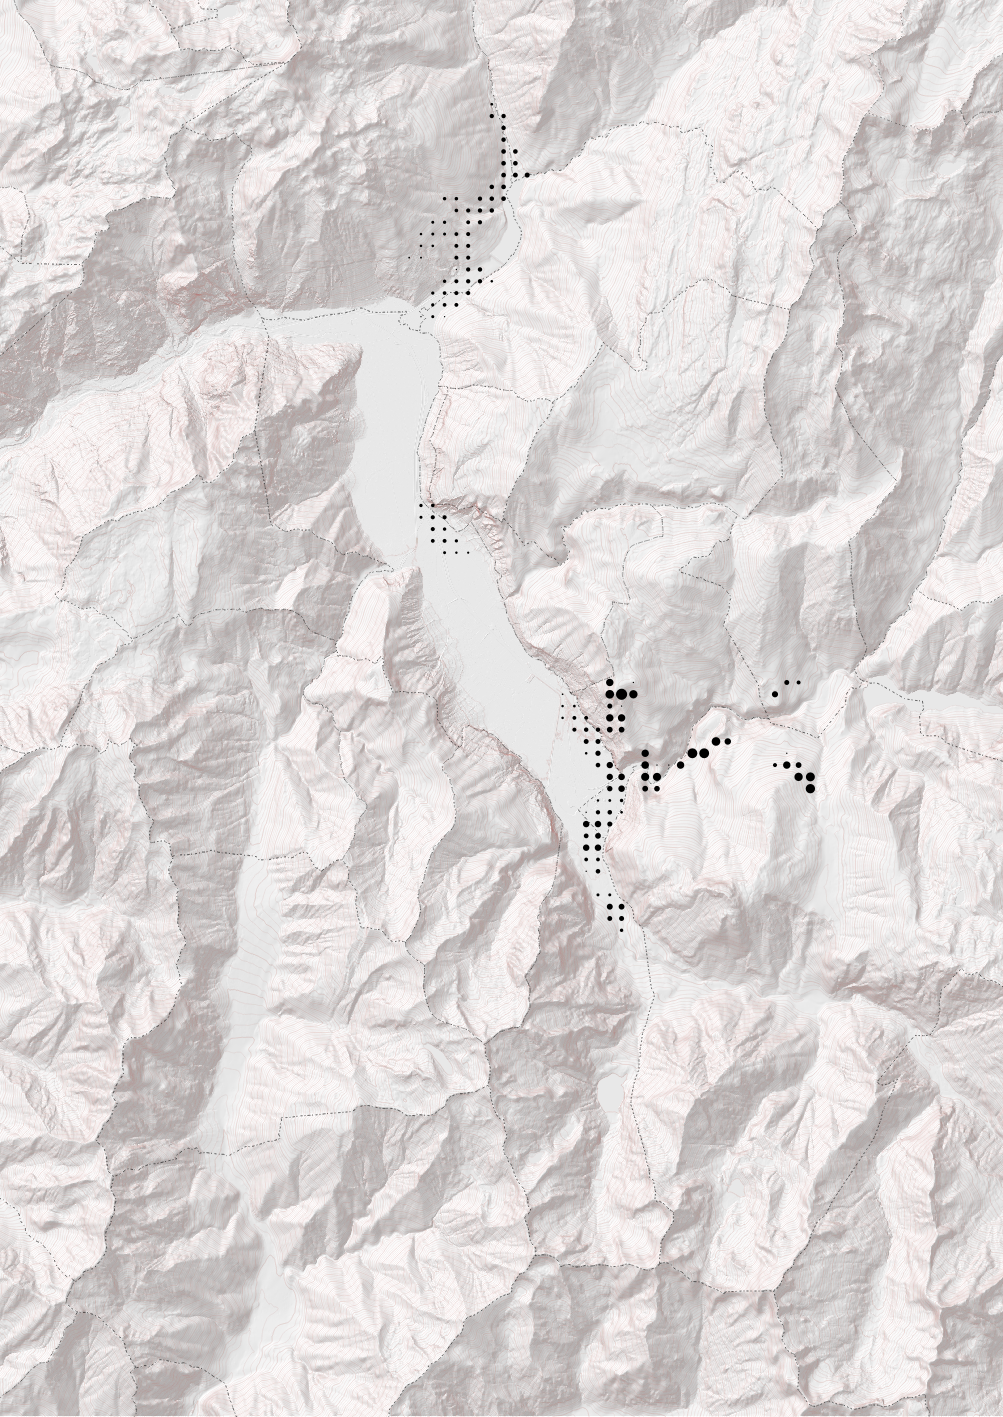
\includegraphics{./figures/CarteTest5.png}};
      \begin{scope}
        \node (P2) at ([yshift=-.5cm]image.south east) {};
        \node (P1) at ([yshift=-.5cm]image.south west) {};
        % Échelle
        \draw[-] (P2 |- 0,-1) --++ (-1,0) node[pos=.5, above] {\SI{2,5}{\kilo\meter}};
      \end{scope}
    \end{tikzpicture}
  \end{center}
  \caption{Représentation de la}
  \label{fig:1}
\end{carte}

\Blindtext

\section{Le projet Choucas}

\begin{table}
  \centering
  \begin{tabular}{ l !{$\rightarrow$} l} 
    \hline
    Nombre & \num{24415.15625}\\
    Nombre arrondi & \num[round-precision=1]{24415.15625}\\
    Nombre arrondi & \SI[round-precision=1]{24415.15625}{\%}\\
    Nombres & \num{10240x7680} \\
    Angle & \ang{234} \\
    Unité composite & \SI{210}{\km\per\hour} \\
    Plage & \SIrange{10}{25}{\liter} \\
    Liste & \SIlist{0;8;16;32;64}{\mega b} \\

  \end{tabular}
  \caption{test array}
\end{table}


\begin{figure}
  \begin{center}
    \subimport{figures/}{canevas.tikz}
  \end{center}
  \caption{Représentation de la}
  \label{fig:1}
\end{figure}

\begin{table}
  \centering
  \begin{tabular}{ l !{$\rightarrow$} l} 
    \hline
    Nombre & \num{24415.15625}\\
    Nombre arrondi & \num[round-precision=1]{24415.15625}\\
    Nombre arrondi & \SI[round-precision=1]{24415.15625}{\%}\\
    Nombres & \num{10240x7680} \\
    Angle & \ang{234} \\
    Unité composite & \SI{210}{\km\per\hour} \\
    Plage & \SIrange{10}{25}{\liter} \\
    Liste & \SIlist{0;8;16;32;64}{\mega b} \\
  \end{tabular}
  \caption{test array 2}
\end{table}

\begin{carte}
  \begin{center}
    \subimport{figures/}{canevas.tikz}
  \end{center}
  \caption{Représentation de la}
  \label{map:1}
\end{carte}

\addsec{Conclusion}

Conclusion du chapitre

%%% Local Variables:
%%% mode: lualatex
%%% TeX-master: "../main"
%%% End:
